
\begin{figure}[ht]
  \begin{widepage}
    \centering
    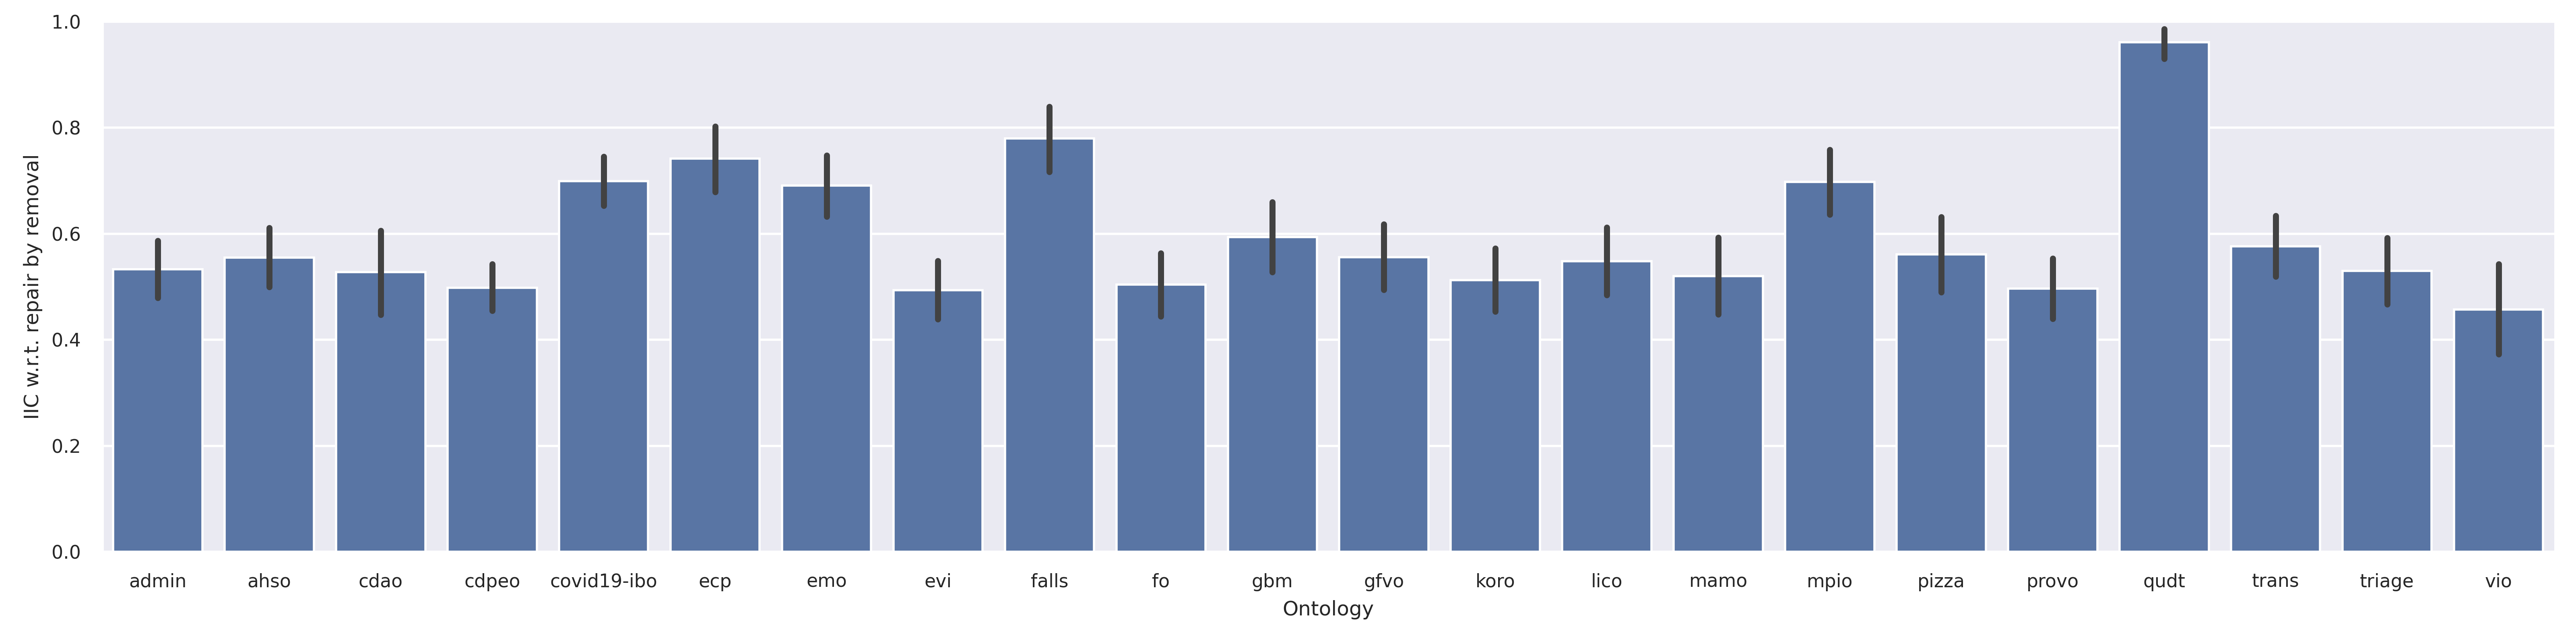
\includegraphics[width=\textwidth]{resources/iic-remove-ontology-bar.png}
  \end{widepage}
  \caption{Mean IIC with respect to repair via removal per ontology. The error bars show the 95\% confidence interval.}
\end{figure}

\begin{figure}[ht]
\begin{widepage}
  \centering
  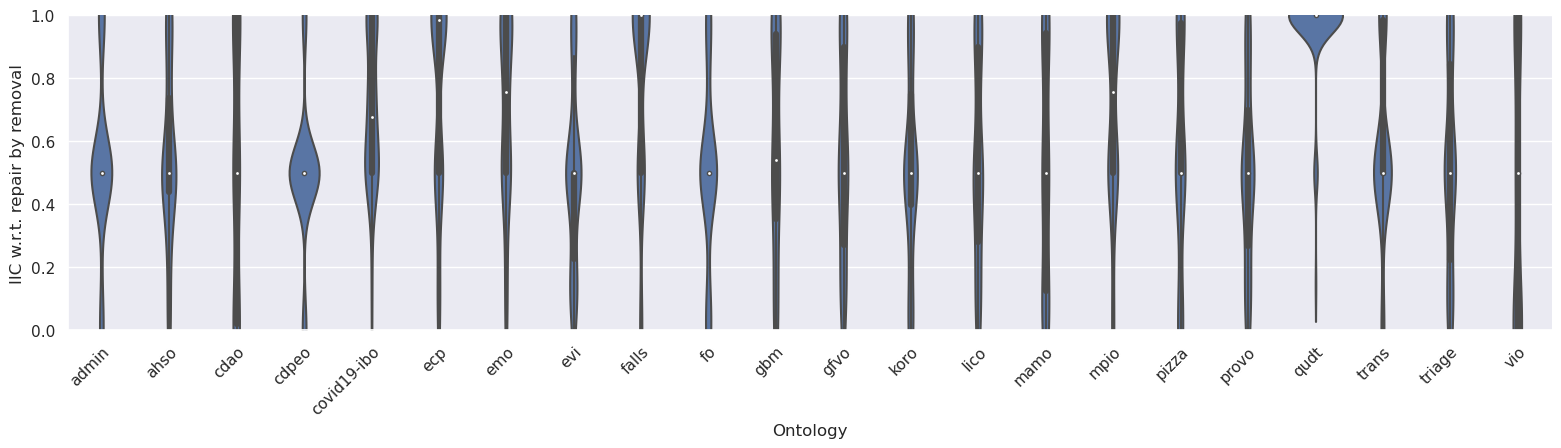
\includegraphics[width=\textwidth]{resources/iic-remove-ontology-violin.png}
\end{widepage}
\caption{Distribution of IIC with respect to repair via removal per ontology.}
\end{figure}

\begin{figure}[ht]
  \begin{widepage}
    \centering
    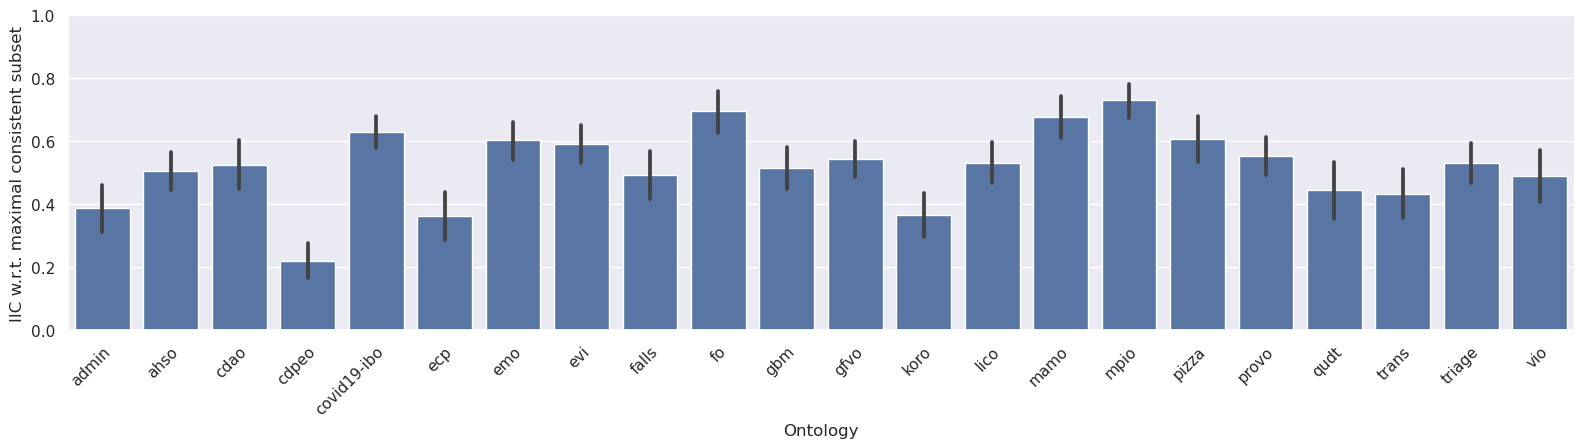
\includegraphics[width=\textwidth]{resources/iic-mcs-ontology-bar.png}
  \end{widepage}
  \caption{Mean IIC with respect to repair via a random maximal consistent subset per ontology. The error bars show the 95\% confidence interval.}
\end{figure}

\begin{figure}[ht]
    \begin{widepage}
      \centering
      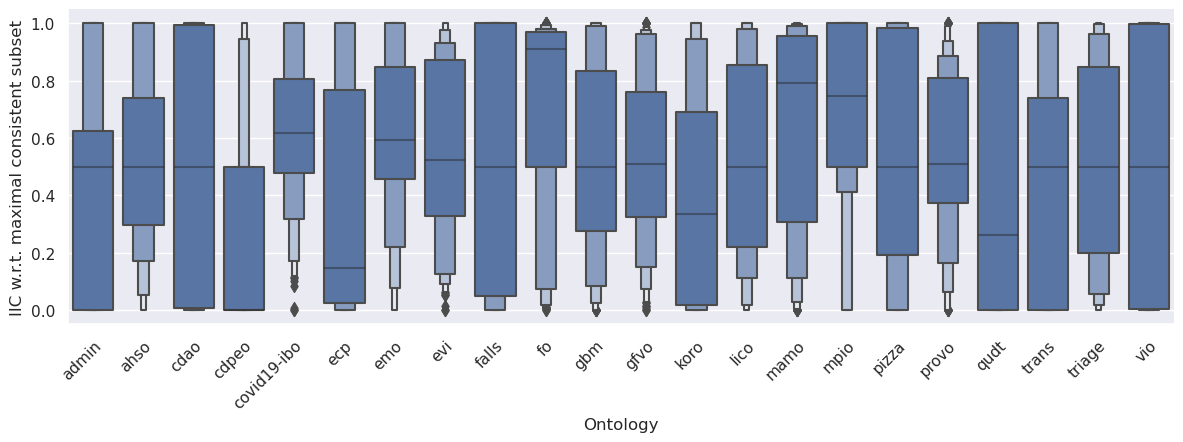
\includegraphics[width=\textwidth]{resources/iic-mcs-ontology-violin.png}
    \end{widepage}
    \caption{Distribution of IIC with respect to repair via a random maximal consistent subset per ontology.}
\end{figure}

\begin{figure}[ht]
    \begin{widepage}
      \centering
      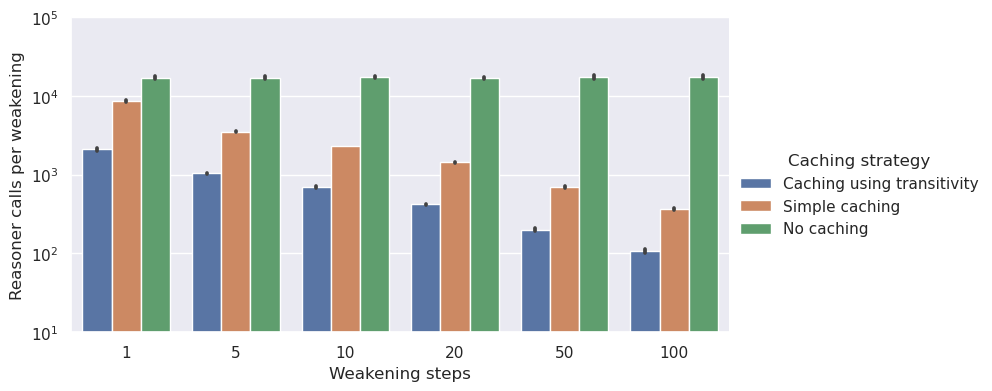
\includegraphics[width=\textwidth]{resources/calls-cache-bar.png}
    \end{widepage}
    \caption{Average reasoner calls with different caching strategies when executing axiom weakening of random axioms. Results are the average between the following ontologies: admin, cdpeo, emo, gbm, gfvo, koro, and mamo. Each consistency or entailment query made to the reasoner count as one call.}
\end{figure}

\begin{figure}[ht]
    \begin{widepage}
      \centering
      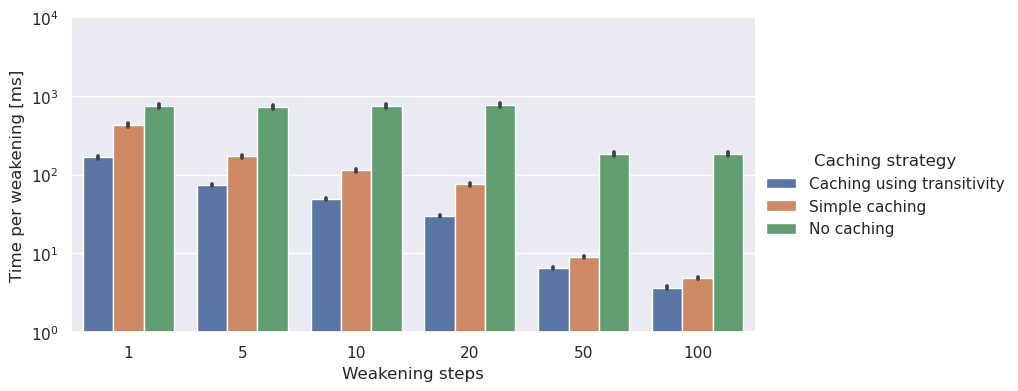
\includegraphics[width=\textwidth]{resources/time-cache-bar.png}
    \end{widepage}
    \caption{Average time required per application of the axiom weakening operator with different caching strategies when executing axiom weakening of random axioms. Results are the average between the following ontologies: admin, cdpeo, emo, gbm, gfvo, koro, and mamo. The results are averaged for the reasoners FaCT++, JFact, Openllet, and HermiT.}
\end{figure}

\begin{figure}[ht]
    \begin{widepage}
      \centering
      
\includegraphics[height=0.9\textheight]{resources/calls-cache-ontology-bar.png}
    \end{widepage}
    \caption{Average reasoner calls with different caching strategies when executing axiom weakening of random axioms per ontology. Each consistency or entailment query made to the reasoner count as one call.}
\end{figure}

\begin{figure}[ht]
    \begin{widepage}[3cm]
      \centering
      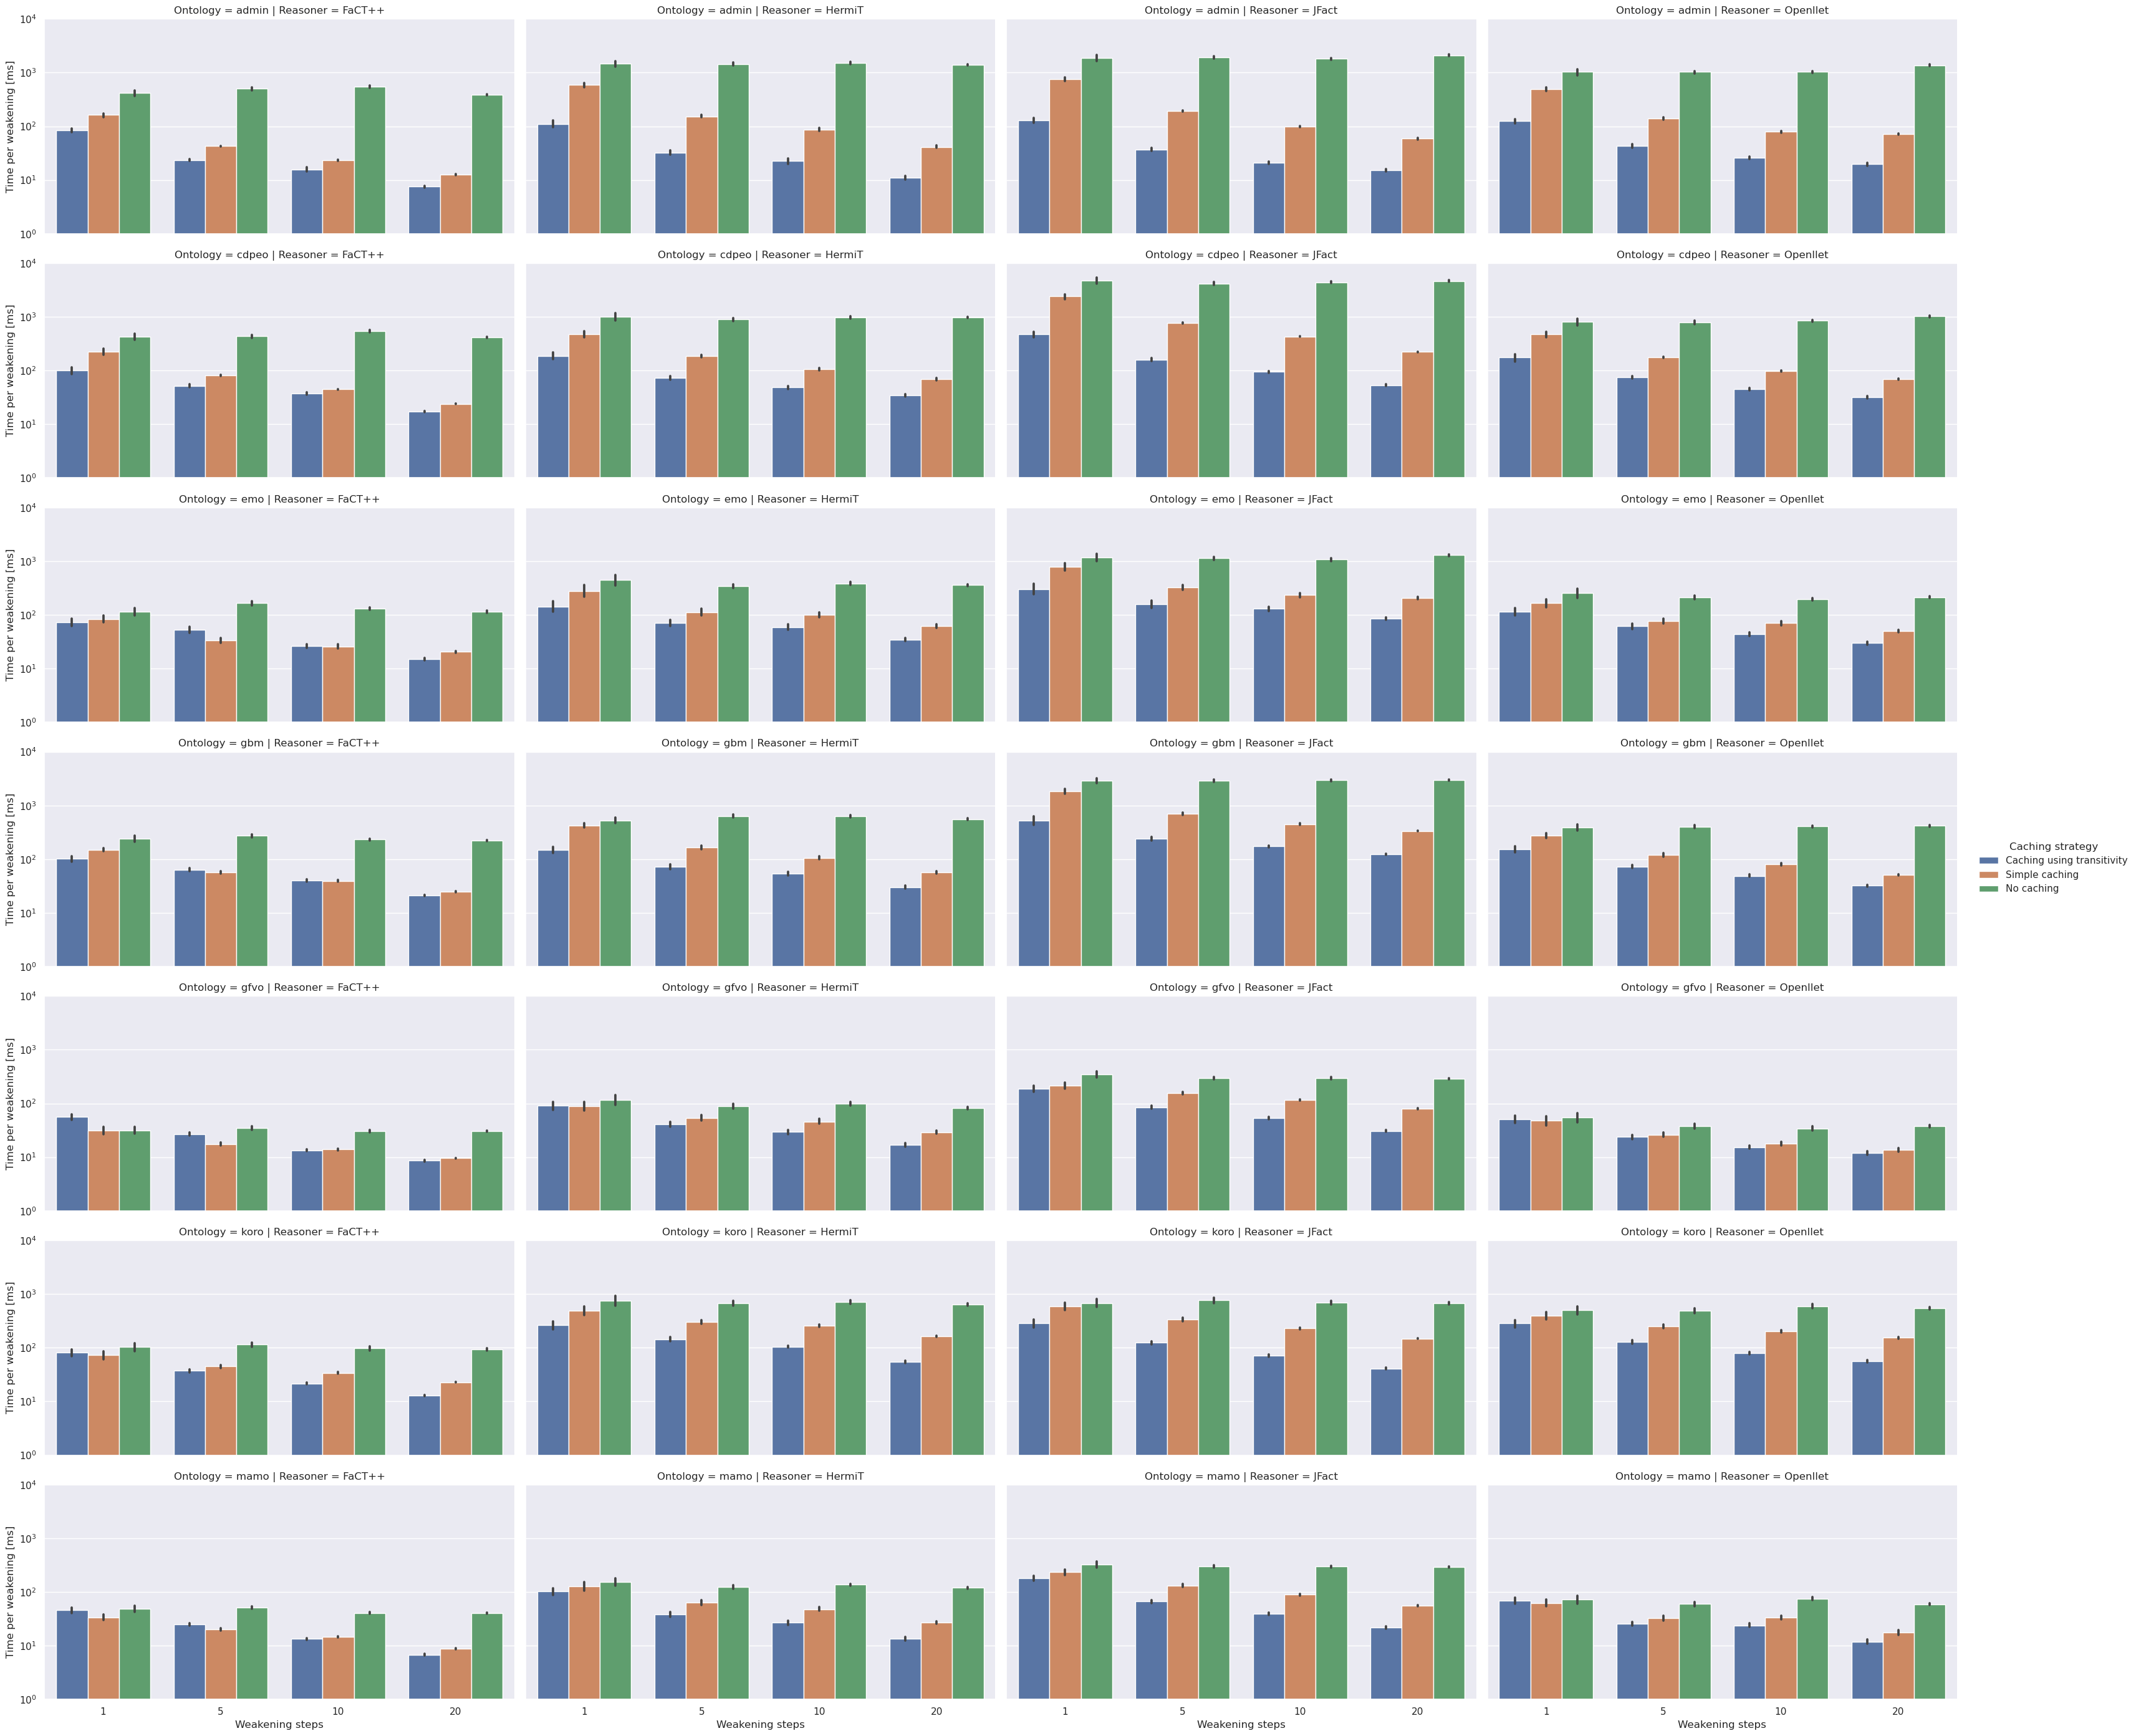
\includegraphics[width=\textwidth]{resources/time-cache-ontology-reasoner-bar.png}
    \end{widepage}
    \caption{Average time required per application of the axiom weakening operator with different caching strategies when executing axiom weakening of random axioms per ontology and reasoner.}
\end{figure}

\begin{table}[ht]
  \scriptsize
  \begin{widepage}[5cm]
    \centering
    \addtolength{\tabcolsep}{-1mm}
    \begin{tabular}{|l|rrrrrr|rrrrrr|rrrrrr|}
      \cline{2-19}
      \multicolumn{1}{l|}{} & \multicolumn{18}{c|}{\hspace{-9mm}Reasoner calls per weakening} \\
      \multicolumn{1}{l|}{} & \multicolumn{6}{c}{Caching using transitivity} & \multicolumn{6}{c}{Simple caching} & \multicolumn{6}{c|}{No caching} \\
      \multicolumn{1}{l|}{} & \multicolumn{1}{c}{1} & \multicolumn{1}{c}{5} & \multicolumn{1}{c}{10} & \multicolumn{1}{c}{20} & \multicolumn{1}{c}{50} & \multicolumn{1}{c}{100} & \multicolumn{1}{c}{1} & \multicolumn{1}{c}{5} & \multicolumn{1}{c}{10} & \multicolumn{1}{c}{20} & \multicolumn{1}{c}{50} & \multicolumn{1}{c}{100} & \multicolumn{1}{c}{1} & \multicolumn{1}{c}{5} & \multicolumn{1}{c}{10} & \multicolumn{1}{c}{20} & \multicolumn{1}{c}{50} & 100 \\
      \hline
      admin & 1096 & 381 & 222 & 131 & 64 & 35
        & 15138 & 4072 & 2115 & 1092 & 459 & 236
        & 41105 & 42224 & 41288 & 41376 & 42663 & 41751 \\
      cdpeo & 2110 & 869 & 522 & 301 & 136 & 75
        & 13621 & 4936 & 2694 & 1436 & 608 & 312
        & 29051 & 27289 & 28617 & 28818 & 28244 & 29315 \\
      emo & 2652 & 1720 & 1355 & 864 & 463 & 258
        & 7781 & 3436 & 2784 & 2023 & 1103 & 619
        & 12524 & 12357 & 12134 & 12548 & 12462 & 12552 \\
      gbm & 3019 & 1577 & 1074 & 674 & 309 & 168
        & 12572 & 5065 & 3284 & 2057 & 956 & 503
        & 19490 & 20945 & 21330 & 20581 & 20780 & 20801 \\
      gfvo &  1737 & 891 & 575 & 335 & 151 & 80
        & 2828 & 1975 & 1524 & 1043 & 539 & 293
        & 4058 & 3973 & 4104 & 4012 & 3977 & 4003 \\
      koro & 2006 & 952 & 591 & 344 & 157 & 80
        & 5154 & 3046 & 2272 & 1465 & 721 & 382
        & 7271 & 7618 & 7181 & 7223 & 7233 & 7422 \\
      mamo &  1984 & 844 & 511 & 286 & 122 & 61
        & 3557 & 2140 & 1488 & 943 & 449 & 234
        & 5060 & 5011 & 5059 & 5037 & 4997 & 4998 \\
      \hline
      Overall & 2086 & 1033 & 693 & 419 & 200 & 108
        & 8664 & 3524 & 2309 & 1437 & 691 & 368
        & 16937 & 17059 & 17102 & 17007 & 17194 & 17263 \\
      \hline
    \end{tabular}
  \end{widepage}
  \caption{Results of the evaluation of cache effectiveness. The mean number of reasoner calls required for a single weakening is given.}
\end{table}

\begin{table}[ht]
  \scriptsize
  \begin{widepage}[4cm]
    \centering
    \addtolength{\tabcolsep}{-1mm}
    \begin{tabular}{|l|l|rrrrrr|rrrrrr|rrrrrr|}
      \cline{3-20}
      \multicolumn{2}{l|}{} & \multicolumn{18}{c|}{\hspace{-6mm}Time per weakening [ms]} \\
      \multicolumn{2}{l|}{} & \multicolumn{6}{c}{Caching using transitivity} & \multicolumn{6}{c}{Simple caching} & \multicolumn{6}{c|}{No caching} \\
      \multicolumn{2}{l|}{} & \multicolumn{1}{c}{1} & \multicolumn{1}{c}{5} & \multicolumn{1}{c}{10} & \multicolumn{1}{c}{20} & \multicolumn{1}{c}{50} & \multicolumn{1}{c}{100} & \multicolumn{1}{c}{1} & \multicolumn{1}{c}{5} & \multicolumn{1}{c}{10} & \multicolumn{1}{c}{20} & \multicolumn{1}{c}{50} & \multicolumn{1}{c}{100} & \multicolumn{1}{c}{1} & \multicolumn{1}{c}{5} & \multicolumn{1}{c}{10} & \multicolumn{1}{c}{20} & \multicolumn{1}{c}{50} & 100 \\
      \hline
      \multirow{8}{*}{FaCT++} & admin
        & 83.6 & 23.6 & 15.7 & 7.5 & 4.2 & 2.6
        & 162.1 & 42.8 & 23.3 & 12.6 & 5.8 & 3.2
        & 416.8 & 503.9 & 543.6 & 389.4 & 389.5 & 369.1 \\
      & cdpeo
        & 99.6 & 52.2 & 37.5 & 17.1 & 8.9 & 5.4
        & 227.6 & 81.0 & 44.8 & 24.0 & 11.4 & 6.4
        & 429.3 & 437.3 & 540.7 & 413.8 & 397.8 & 409.3 \\
      & emo
        & 72.2 & 52.3 & 26.5 & 15.0 & 8.3 & 4.7
        & 83.8 & 33.4 & 25.9 & 20.4 & 11.8 & 6.9
        & 113.4 & 164.3 & 131.1 & 114.0 & 110.9 & 108.0 \\
      & gbm
        & 101.6 & 63.3 & 39.9 & 21.1 & 10.8 & 5.8
        & 150.2 & 56.6 & 39.5 & 24.8 & 12.2 & 6.4
        & 240.7 & 272.0 & 232.5 & 220.3 & 218.5 & 217.7 \\
      & gfvo
        & 55.7 & 26.8 & 13.3 & 8.6 & 4.2 & 2.2
        & 31.5 & 17.6 & 13.9 & 9.5 & 5.1 & 2.7
        & 31.6 & 35.0 & 30.4 & 30.7 & 30.1 & 29.7 \\
      & koro
        & 81.3 & 37.0 & 21.5 & 12.8 & 6.2 & 3.4
        & 72.9 & 45.0 & 34.0 & 22.7 & 11.6 & 6.2
        & 103.0 & 114.6 & 97.0 & 93.9 & 93.9 & 94.0 \\
      & mamo
        & 45.7 & 24.8 & 13.3 & 6.8 & 3.3 & 1.6
        & 33.8 & 20.2 & 14.6 & 8.8 & 4.5 & 2.4
        & 48.8 & 51.0 & 40.7 & 40.4 & 40.6 & 42.1 \\
      \cline{2-20}
      & Overall
        & 77.1 & 40.0 & 24.0 & 12.7 & 6.5 & 3.7
        & 108.8 & 42.4 & 28.0 & 17.6 & 8.9 & 4.9
        & 197.7 & 225.5 & 230.9 & 186.1 & 183.0 & 181.4 \\
      \hline
      \multirow{8}{*}{HermiT} & admin
        & 111.0 & 32.4 & 22.4 & 11.1 & &
        & 585.2 & 152.5 & 86.9 & 41.3 & &
        & 1469.9 & 1448.1 & 1519.6 & 1388.0 & & \\
      & cdpeo
        & 187.1 & 73.2 & 48.5 & 34.2 & &
        & 481.1 & 186.0 & 105.7 & 68.5 & &
        & 1017.3 & 894.3 & 984.6 & 975.8 & & \\
      & emo
        & 143.0 & 71.4 & 59.3 & 34.5 & &
        & 275.7 & 112.3 & 100.9 & 61.3 & &
        & 444.0 & 342.3 & 384.3 & 358.4 & & \\
      & gbm
        & 149.0 & 72.2 & 53.4 & 30.1 & &
        & 424.9 & 164.8 & 105.6 & 56.1 & &
        & 523.8 & 632.9 & 629.5 & 557.5 & & \\
      & gfvo
        & 90.1 & 40.4 & 29.3 & 16.8 & &
        & 89.2 & 54.0 & 46.0 & 28.9 & &
        & 115.2 & 87.7 & 97.8 & 81.5 & & \\
      & koro
        & 264.8 & 144.6 & 104.3 & 54.3 & &
        & 494.7 & 303.7 & 255.8 & 163.6 & &
        & 752.9 & 676.2 & 702.3 & 634.4 & & \\
      & mamo
        & 102.0 & 38.5 & 26.7 & 13.3 & &
        & 128.0 & 63.0 & 47.8 & 26.8 & &
        & 154.0 & 124.3 & 136.5 & 119.9 & & \\
      \cline{2-20}
      & Overall
        & 149.6 & 67.5 & 49.1 & 27.8 & &
        & 354.1 & 148.0 & 106.9 & 63.8 & &
        & 639.6 & 600.8 & 636.4 & 587.9 & & \\
      \hline
      \multirow{8}{*}{JFact} & admin
        & 128.1 & 37.1 & 21.0 & 15.1 & &
        & 751.6 & 193.2 & 99.3 & 58.9 & &
        & 1877.9 & 1938.7 & 1806.7 & 2109.6 & & \\
      & cdpeo
        & 472.1 & 160.3 & 95.4 & 53.6 & &
        & 2404.9 & 775.5 & 428.3 & 222.5 & &
        & 4764.2 & 4193.6 & 4432.1 & 4657.4 & & \\
      & emo
        & 302.1 & 157.9 & 129.2 & 85.0 & &
        & 781.9 & 327.1 & 233.9 & 205.3 & &
        & 1170.6 & 1126.2 & 1068.0 & 1295.2 & & \\
      & gbm
        & 520.1 & 238.1 & 172.2 & 123.1 & &
        & 1834.8 & 701.8 & 447.9 & 335.0 & &
        & 2862.4 & 2878.8 & 2965.3 & 2981.6 & & \\
      & gfvo
        & 189.3 & 84.7 & 53.5 & 30.5 & &
        & 215.4 & 155.4 & 116.4 & 79.4 & &
        & 345.7 & 294.1 & 293.3 & 290.1 & & \\
      & koro
        & 286.4 & 123.8 & 71.2 & 41.0 & &
        & 595.5 & 333.6 & 228.6 & 148.4 & &
        & 681.2 & 763.0 & 696.3 & 678.9 & & \\
      & mamo
        & 181.3 & 66.8 & 39.0 & 21.7 & &
        & 234.2 & 132.4 & 89.7 & 55.4 & &
        & 328.3 & 296.1 & 298.7 & 291.1 & & \\
      \cline{2-20}
      & Overall
        & 297.1 & 124.1 & 83.1 & 52.8 & &
        & 974.1 & 374.1 & 234.9 & 157.8 & &
        & 1718.6 & 1641.5 & 1651.5 & 1757.7 & & \\
      \hline
      \multirow{8}{*}{Openllet} & admin
        & 125.0 & 42.7 & 25.9 & 19.7 & &
        & 489.5 & 138.9 & 79.2 & 71.3 & &
        & 1026.0 & 1026.5 & 1028.9 & 1376.1 & & \\
      & cdpeo
        & 175.3 & 74.9 & 45.4 & 31.7 & &
        & 472.0 & 176.9 & 97.7 & 68.9 & &
        & 815.7 & 795.5 & 845.0 & 1025.4 & & \\
      & emo
        & 113.0 & 61.0 & 43.8 & 29.7 & &
        & 165.6 & 77.4 & 69.8 & 49.9 & &
        & 252.5 & 210.6 & 197.3 & 212.2 & & \\
      & gbm
        & 153.5 & 73.0 & 48.9 & 32.0 & &
        & 276.2 & 120.5 & 79.7 & 51.2 & &
        & 391.4 & 403.7 & 406.6 & 418.1 & & \\
      & gfvo
        & 50.4 & 23.8 & 15.4 & 11.9 & &
        & 47.8 & 26.3 & 17.8 & 13.5 & &
        & 54.6 & 37.9 & 34.1 & 37.5 & & \\
      & koro
        & 282.5 & 127.2 & 79.2 & 55.3 & &
        & 399.2 & 250.2 & 202.6 & 152.6 & &
        & 499.9 & 491.9 & 595.2 & 549.4 & & \\
      & mamo
        & 68.8 & 25.6 & 23.9 & 11.8 & &
        & 62.2 & 32.6 & 33.2 & 17.4 & &
        & 71.7 & 59.6 & 75.1 & 58.9 & & \\
      \cline{2-20}
      & Overall
        & 138.3 & 61.2 & 40.3 & 27.4 & &
        & 273.2 & 117.5 & 82.9 & 60.7 & &
        & 444.5 & 432.2 & 454.6 & 514.3 & & \\
      \hline
    \end{tabular}
  \end{widepage}
  \caption{Results of the evaluation of cache effectiveness. The mean execution time required for a single weakening is given.}
\end{table}

\begin{figure}[ht]
  \begin{widepage}
    \centering
    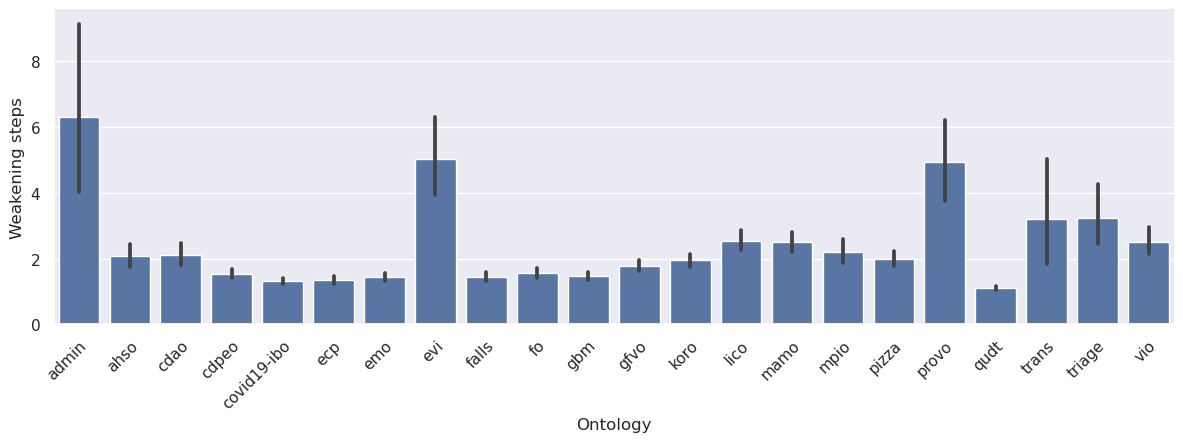
\includegraphics[width=\textwidth]{resources/steps-ontology-bar.png}
  \end{widepage}
  \caption{Mean number of weakening steps needed for repairing the ontology. The error bars show the 95\% confidence interval.}
\end{figure}

\begin{figure}[ht]
  \begin{widepage}
    \centering
    \begin{subfigure}[T]{0.175\textwidth}
      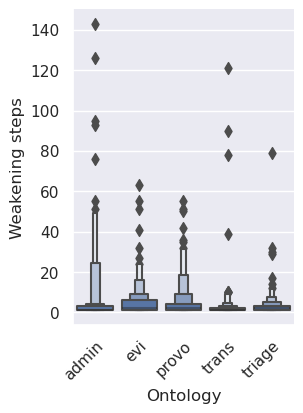
\includegraphics[width=\textwidth]{resources/steps-ontology-violin-1.png}
    \end{subfigure}
    \begin{subfigure}[T]{0.77\textwidth}
      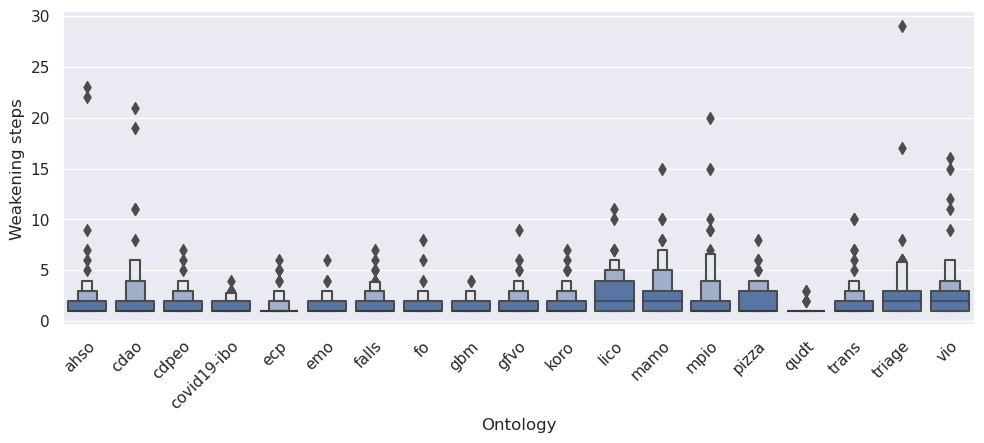
\includegraphics[width=\textwidth]{resources/steps-ontology-violin-2.png}
    \end{subfigure}
  \end{widepage}
  \caption{Distribution of required weakening steps for repairing using axiom weakening by ontology. Attempts that failed by timeout were not considered.}
\end{figure}

\begin{figure}[ht]
  \begin{widepage}
    \centering
    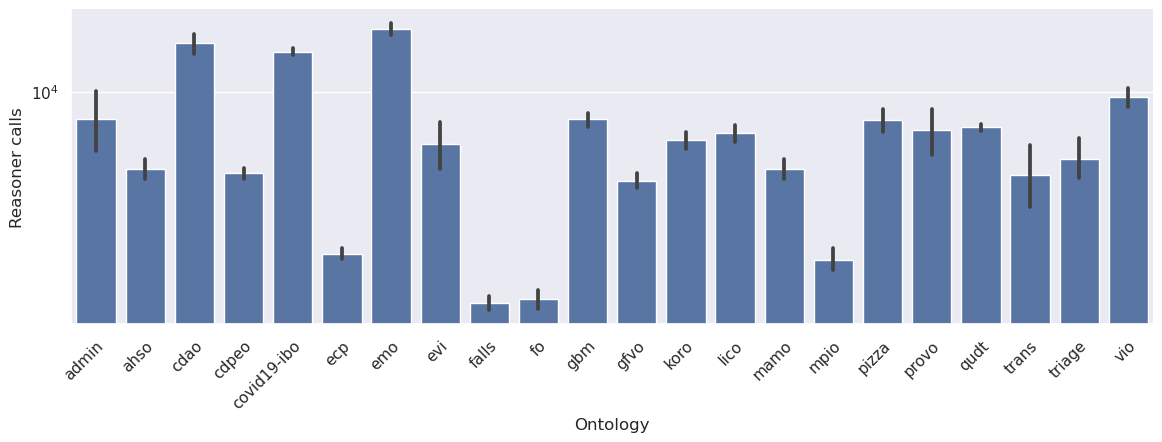
\includegraphics[width=\textwidth]{resources/calls-ontology-bar.png}
  \end{widepage}
  \caption{Mean number of reasoner calls required for repairing using axiom weakening by ontology. The error bars show the 95\% confidence interval. Attempts that failed by timeout were not considered.}
\end{figure}

\begin{figure}[ht]
  \begin{widepage}
    \centering
    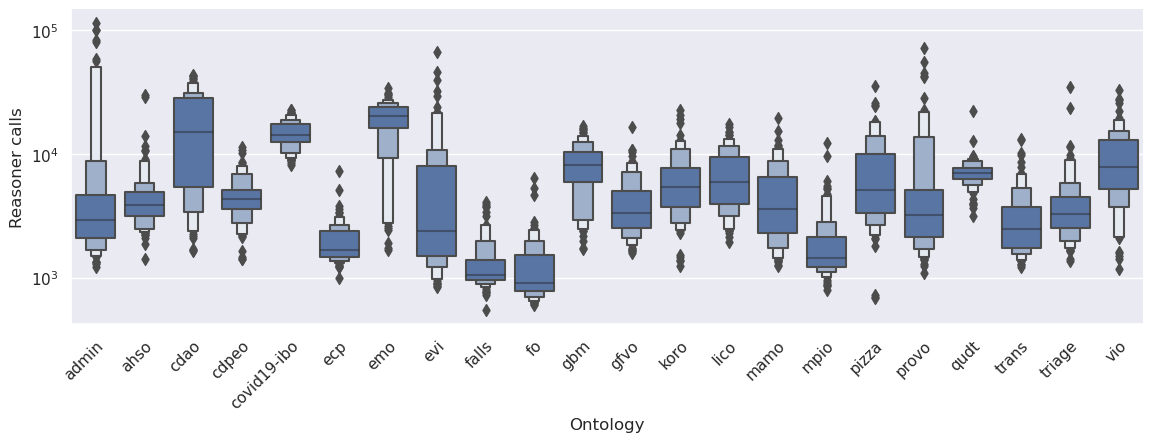
\includegraphics[width=\textwidth]{resources/calls-ontology-violin.png}
  \end{widepage}
  \caption{Distribution of reasoner calls required for repairing using axiom weakening by ontology. Attempts that failed by timeout were not considered.}
\end{figure}

\begin{figure}[ht]
  \begin{widepage}
    \centering
    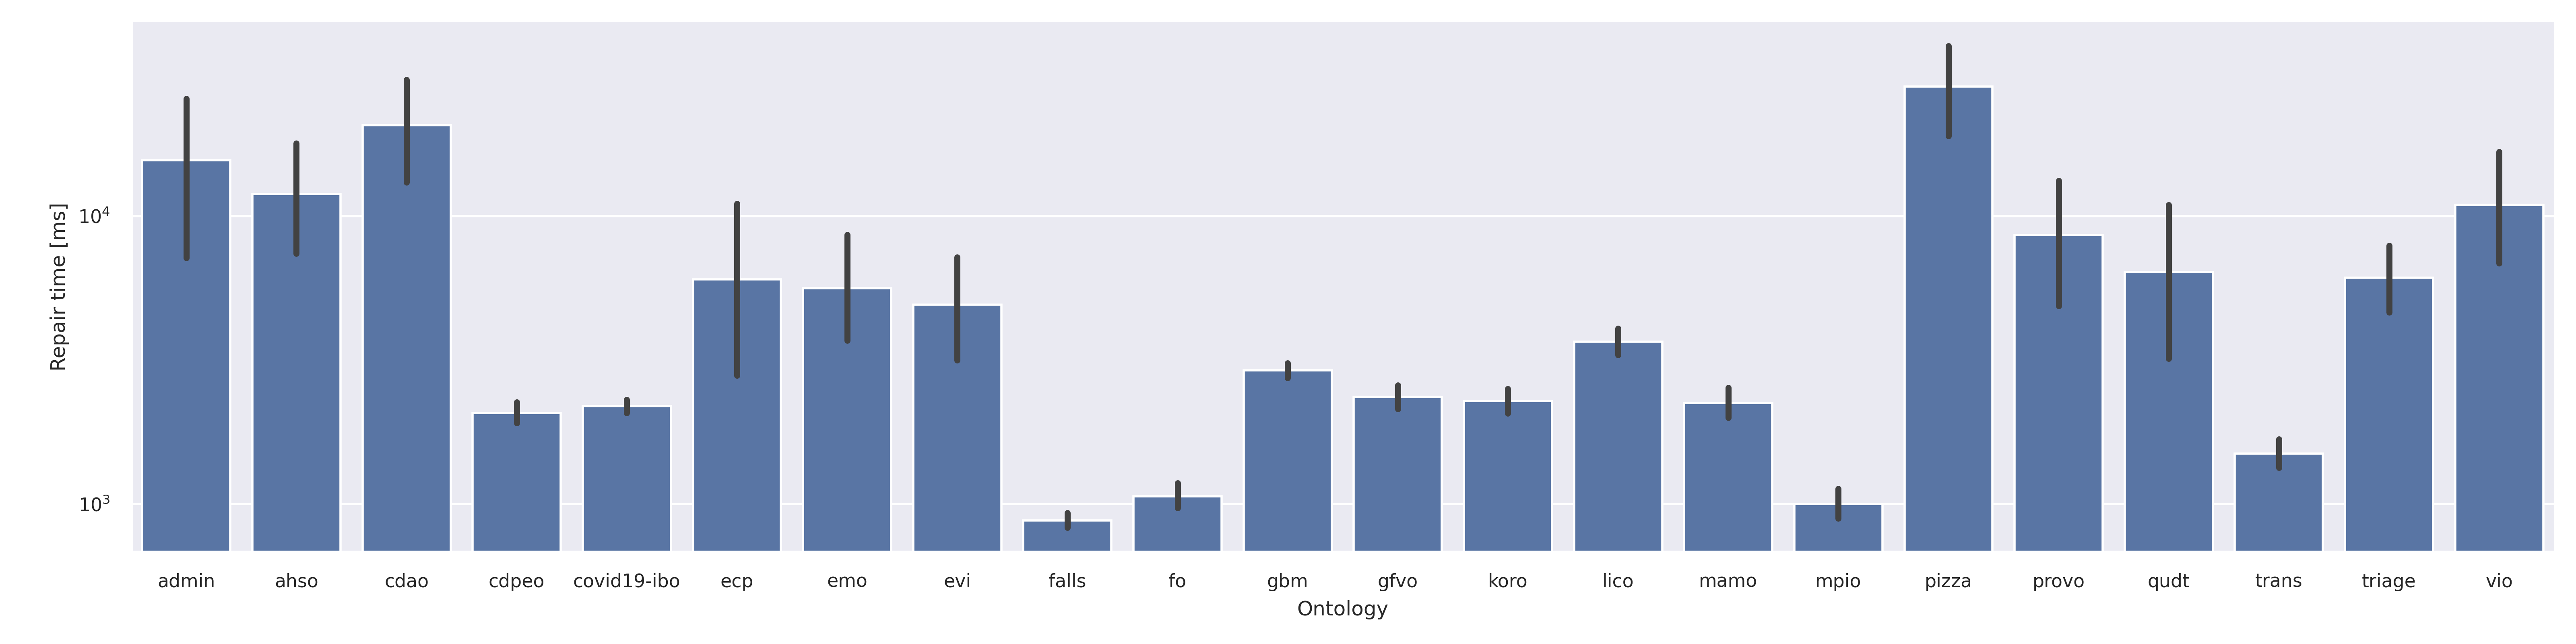
\includegraphics[width=\textwidth]{resources/time-ontology-bar.png}
  \end{widepage}
  \caption{Mean execution time required for repairing using axiom weakening by ontology. The error bars show the 95\% confidence interval. Attempts that failed by timeout were not considered.}
\end{figure}

\begin{figure}[ht]
  \begin{widepage}
    \centering
    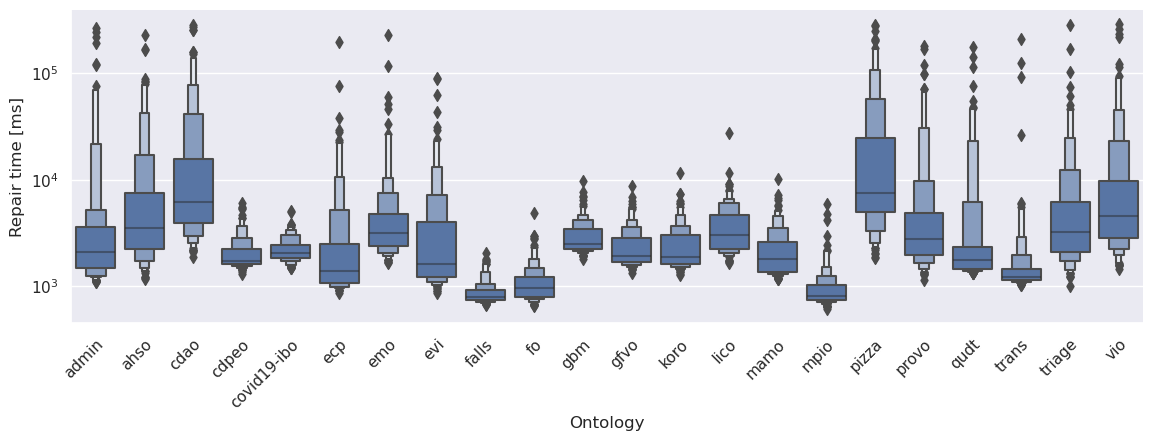
\includegraphics[width=\textwidth]{resources/time-ontology-violin.png}
  \end{widepage}
  \caption{Distribution of execution time required for repairing using axiom weakening by ontology. Attempts that failed by timeout were not considered.}
\end{figure}
